\section{Methods} \label{s:methods}

\subsection{FFT database} \label{ss:m-fft-database} 

This study is a reanalysis of data collected as part of the NASA Forest
Functional Types (FFT) campaign.  The data contains 1348 leaf reflectance and
transmittance spectra (ASD Fieldspec 3 Full Range Spectroradiometer,
\SIrange{350}{2500}{\nano\meter}, interpolated at \SI{1}{\nano\meter})
collected from various positions in the canopy for 52 species from 13 sites
across the Northeast and Midwest USA. For 950 of these leaves, additional
laboratory measurements of leaf mass per unit area (LMA) and equivalent water
thickness (EWT) were performed. For further information on the sampling
methodology, see \cite{Singh2015}.

\subsection{PROSPECT 5 model} \label{ss:m-prospect5}

The PROSPECT 5 model simulates the full reflectance spectrum of a leaf over
the range \SIrange{400}{2500}{\nano\meter} using five parameters related to
leaf structure and biochemistry: N, the effective number of leaf plates (see
below); Cab, the chlorophyll (\em{a} and \em{b}) content per unit area
(\si{\micro\gram\per\square\centi\meter}); Car, the carotenoid (anthocyanin,
xanthophyll) content per unit area (\si{\micro\gram\per\square\centi\meter});
Cw, the equivalent water thickness (\si{\centi\meter}); and Cm, the leaf dry
matter content per unit area (\si{\gram\per\square\centi\meter}). A leaf is
treated as a set of partially transparent flat plates, with the transmissivity
of each plate based on the linear combination of predefined specific
absorption spectra for water, chlorophyll, carotenoids, and dry matter (e.g.
cellulose, lignin) multiplied by their respective quantities (i.e. the
parameter values: Cab, Car, Cw, Cm) (Figure \ref{fig:prospectsens}). For
further detail, see \cite{Jacquemoud1990, Feret2008}.

\begin{figure}[h]
  \centerline{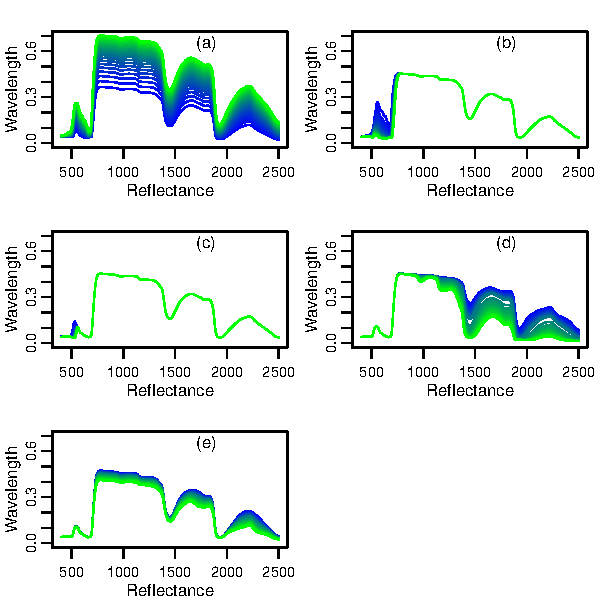
\includegraphics{figures/sensitivity}}
  \caption{
  Sensitivity of PROSPECT modeled reflectance to parameter values: (a) N, (b) 
  Cab, (c) Car, (d) Cw, and (e) Cm. Values increase from blue to green.
  }
  \label{fig:prospectsens}
\end{figure}

\subsection{Inversion procedure} \label{ss:m-inversion}

The complexity and non-linearity of the PROSPECT 5 model precludes an 
analytical solution for the parameters as a function of reflectance. Instead, 
we performed a statistical inversion, wherein the residual error between 
modeled and observed reflectance is modeled. This analysis was performed 
within a Bayesian framework, such that the result was a joint probability 
distribution of each PROSPECT 5 parameter and the residual error informed by 
prior expectations. The general mathematical statement of this posterior 
distribution is given as follows:

\begin{align}
  P(\theta, \sigma | \mathbf{X}) &\propto P(\mathbf{X} | \theta, \sigma) 
  P(\theta) P(\sigma) \\
  P(\mathbf{X} | \theta, \sigma) &= \mathit{Normal}(\mathrm{PROSPECT 5}(\theta) | \mathbf{X}, \sigma)
  \label{eq:bayes}
\end{align}

, where $\theta$ is the vector of PROSPECT 5 parameters, $\sigma$ is the 
residual standard deviation, $\mathrm{PROSPECT 5}(\theta)$ is the simulated
reflectance given $\theta$, and $\mathbf{X}$ is a vector of observed 
reflectance values. The residual error is assumed to be normally distributed 
with a mean of 0 and standard deviation $\sigma$. 

We set prior distributions on the PROSPECT 5 parameters to accommodate their
strict lower bounds (1 for N, 0 for Cab, Car, Cw, and Cm) while maintaining
approximately equal and low probability density over the entire range of
realistic values. We set the prior distribution for N to a lognormal
distribution shifted horizontally to have a minimum at 1 and parameterized
based on a review of literature featuring the PROSPECT model (e.g.
\cite{LeMaire2004,Ferreira2013,Croft2014}). We assigned the remaining
parameters log-normal priors based on summary statistics and histograms from
four spectral databases presented by Feret et al. (\cite{Feret2008}). The
residual variance $\sigma^2$ was assigned an uninformative inverse gamma
prior, which is conjugate with the normal and therefore allows for Gibbs
sampling.

We sampled the joint posterior distribution of the PROSPECT 5 parameters using
the Metropolis-Hastings (MH) algorithm with adaptive block sampling
(\cite{Haario2001}). Samples were drawn from a multivariate normal
distribution with means conditioned on the current accepted values and the
covariance matrix $\mathbf{J}$ re-computed every 100 samples as follows:

\begin{align}
    \mathbf{R} &= \frac{\mathbf{S} \times a}{t} \\
    \mathbf{J} &= \mathbf{R} \times \mathbf{C} \times \mathbf{R}
\end{align}

, where $\mathbf{R}$ is a diagonal matrix of factors for scaling the 
correlation matrix $\mathbf{C}$, $\mathbf{S}$ is a diagonal matrix of the 
sample standard deviations of parameters for the current 100-sample block, $a$ 
is the fraction of samples from the current block that have been accepted, and
$t$ is the target acceptance rate (set to 0.44, as per \cite{Haario2001}).  We
initialized inversions at random values drawn from the prior distributions,
but to improve convergence, these initial values were then optimized using the
Levenberg-Marquhardt (LM) algorithm prior to starting the Metropolis-Hastings
algorithm. Doing this worked for the majority of cases; however, for a small
subset of runs, the LM algorithm picked unrealistically large values (e.g. N >
20, Cab > 1000), causing the subsequent inversion to fail to converge on the
known correct values. When we skipped the initial LM optimization, the
inversion took longer to converge but never failed to converge (results not
shown). We assessed convergence and determined the burn-in period by visually
analyzing trace plots of the MH samples. We determined the thinning interval
by visually examining the autocorrelograms.  For each inversion, we calculated
the mean, standard deviation, median, and 95\% confidence intervals of the
sampled parameter values.  

The inversion algorithm described above is available as an open-source,
publicly-available R (\cite{Rcore}) package housed as a module within the
PEcAn ecoinformatics toolbox
(\url{github.com/PecanProject/PEcAn/modules/rtm}). Our package allows users to
simulate spectra using the PROSPECT and PROSAIL family of radiative transfer
models and apply our inversion algorithm to their own models and data. For
more information, see the package vignette.


\subsection{Validation} \label{ss:m-validation}

We performed two different tests to evaluate the accuracy of our inversion of
measured leaf spectra. First, we used the mean parameter estimates from each
leaf spectrum inversion to generate simulated reflectance and transmittance
spectra and compared these simulations to measured reflectance and
transmittance. The use of transmittance makes this approach robust, as the
inversions were performed on only reflectance data. For both reflectance and
transmittance, we plotted the mean and 90\% and 95\% confidence intervals on
the absolute error (simulated $-$ measured) at each wavelength. To facilitate
comparison with other RTM inversion studies (e.g. \cite{Feret2008,
DiVittorio2009}), we also computed the following statistics aggregated across
the visible (VIS, \SIrange{400}{800}{\nano\meter}) and near-infrared (NIR,
\SIrange{801}{2500}{\nano\meter}) regions of the spectrum: 

\begin{align}
  \mathrm{RMSE} &= \sqrt{\frac{\sum_n{\left(x_{\mathrm{sim}} - x_{\mathrm{obs}} \right)^2}}{n}} \\
  \mathrm{BIAS} &= \frac{\sum_n{\left(x_{\mathrm{sim}} - x_{\mathrm{obs}} \right)}}{n} \\
  \mathrm{SEPC} &= \sqrt{\frac{\sum_n{\left(x_{\mathrm{sim}} - x_{\mathrm{obs}} - \mathrm{BIAS}\right)^2}}{n}} \\
  \mathrm{CV} &= \frac{\mathrm{SEPC}}{x_{\mathrm{obs}}} \\
  \mathrm{RMSFE} &= \sqrt{\frac{\sum_n{\left(\frac{x_{\mathrm{sim}} - x_{\mathrm{obs}}}{x_{\mathrm{obs}}}\right)}}{n}}
\end{align}

, where $x_{\mathrm{sim}}$ is the simulated value (reflectance or
transmittance), $x_{\mathrm{obs}}$ is the observed value, and $n$ is the
number of spectra considered.

Second, we compared the mean inversion estimates for Cw and Cm to measured
values of EWT and LMA, respectively, for leaves where both inversion estimates
and measured values were available. For each, we plotted the measured value
against the inversion estimate and computed the same set of statistics as
above.

During exploratory analysis, we observed strong differences between the
results for broadleaved and needle-leaved species. Therefore, to better
contextualize our results, we performed both validation steps for the entire
data set and separately for broadleaved and needle-leaved species.

\subsection{Exploration of the sensor effect} \label{ss:m-sensor-effect}

To investigate the effect of spectral resolution on inversion accuracy and
precision, we simulated reflectance spectra using the PROSPECT 5 model,
transformed these spectra using the spectral response functions of 11 common
remote sensing platforms (Table \ref{tab:sensor-info}), and attempted to
retrieve the starting parameters from the transformed spectra. (We note that
this was done purely for illustration purposes; studies seeking to perform RTM
inversion on real remote sensing data should use a more complicated RTM that
accounts for canopy structure and possible sun-sensor geometry and atmosphere
rather than a simple leaf RTM as we do here.)  For input parameters, we used
the inversion results from measured spectra, thereby capturing a large range
of ecologically realistic values and preserving inherent covariances between
parameters. We then examined how two characteristics of the inversions varied
between sensors: Inaccuracy ($\alpha$) indicates how closely the mean parameter
estimate matched the true value, and uncertainty ($\pi$) indicates the
uncertainty in the inversion's parameter estimate.

\begin{align}
  \alpha &= \frac{\mu - p}{p} \\
  \pi &= \frac{\sigma}{\mu}
\end{align}

, where $\mu$ is the mean parameter estimate, $\sigma$ is the standard
deviation of the parameter estimate, and $p$ is the true parameter value. We
note that both statistics are normalized to facilitate inter-parameter
comparison. Both metrics were computed for each parameter for each inversion
and then averaged over the full range of results.

% Table of sensor information
% Fri Jul 31 20:36:03 2015
\begin{table}[ht]
  \centerline{
\begin{tabular}{cccccc}
  \hline
  Sensor   &   Bands\tablefootnote{Excluding values outside \SIrange{400}{2500}{\nano\meter} range and panchromatic bands} &   Spectral range (\si{\nano\meter})   &   Bandwidth (\si{\nano\meter})   &   Spatial resolution (\si{\meter})   &   Revisit time (days) \\
  \hline
  AVIRIS NG        &   416   &   \numrange{380}{2510}   &   5                     &   \numrange{0.3}{4.0}   &   On-demand only \\
AVIRIS Classic     &   216   &   \numrange{400}{2500}   &   \SI{10}               &   20                    &   On-demand only \\
CHRIS-Proba        &   62    &   \numrange{410}{1050}   &   \numrange{1.5}{12}    &   36                    &   \numrange{7}{8} \\
Hyperion           &   225   &   \numrange{350}{2500}   &   10                    &   30                    &   16 \\
  Landsat 5 TM     &   6     &   \numrange{450}{2350}   &   \numrange{60}{270}    &   30                    &   16 \\
  Landsat 7 ETM+   &   6     &   \numrange{440}{2350}   &   \numrange{60}{280}    &   30                    &   16 \\
  Landsat 8 OLI    &   8     &   \numrange{435}{2295}   &   \numrange{20}{185}    &   30                    &   16 \\
  MODIS (Terra)    &   7     &   \numrange{459}{2155}   &   \numrange{20}{50}     &   \numrange{250}{500}   &   \numrange{1}{2} \\
  VIIRS            &   10    &   \numrange{402}{2275}   &   \numrange{15}{60}     &   750                   &   \numrange{1}{2} \\
  AVHRR            &   3     &   \numrange{580}{1640}   &   \numrange{100}{275}   &   1090                  &   1 \\
   \hline
\end{tabular}
}
\caption{Spectral, spatial, and temporal characteristics of sensors considered in this study.} 
\label{tab:sensor-info}
\end{table}

The data and R source code for performing all analyses in this study is
publicly available at
\url{github.com/ashiklom/prospect_bayes/sensor-manuscript}. We encourage
 interested readers to replicate our analyses and build on them with their own
data and models.